
%(BEGIN_QUESTION)
% Copyright 2012, Tony R. Kuphaldt, released under the Creative Commons Attribution License (v 1.0)
% This means you may do almost anything with this work of mine, so long as you give me proper credit

Suppose you are sent to troubleshoot a vortex flowmeter equipped with a 4-20 mA output, driving an electronic indicator to display water flow rate.  The vortex flow transmitter is loop-powered, which means it receives the electrical power needed to operate over the same two wires that conduct the signal representing rate of flow.  For some reason the indicator is showing a +125\% flow indication (fully saturated upscale) even though we know there isn't that much water flow going through the flowmeter.  Using a digital multimeter, you measure 24 volts between terminals {\bf J} and {\bf K}:

$$\includegraphics[width=15.5cm]{i01114x01.eps}$$

Identify the likelihood of each specified fault for this circuit.  Consider each fault one at a time (i.e. no coincidental faults), determining whether or not each fault could independently account for {\it all} measurements and symptoms in this circuit.

% No blank lines allowed between lines of an \halign structure!
% I use comments (%) instead, so that TeX doesn't choke.

$$\vbox{\offinterlineskip
\halign{\strut
\vrule \quad\hfil # \ \hfil & 
\vrule \quad\hfil # \ \hfil & 
\vrule \quad\hfil # \ \hfil \vrule \cr
\noalign{\hrule}
%
% First row
{\bf Fault} & {\bf Possible} & {\bf Impossible} \cr
%
\noalign{\hrule}
%
% Another row
Flowmeter failed open &  &  \cr
%
\noalign{\hrule}
%
% Another row
Fuse blown (open) &  &  \cr
%
\noalign{\hrule}
%
% Another row
Open cable between C/D and E/F &  &  \cr
%
\noalign{\hrule}
%
% Another row
250 ohm resistor failed open &  &  \cr
%
\noalign{\hrule}
%
% Another row
Flowmeter failed shorted &  &  \cr
%
\noalign{\hrule}
%
% Another row
Shorted cable between C/D and E/F &  &  \cr
%
\noalign{\hrule}
%
% Another row
Voltage source dead &  &  \cr
%
\noalign{\hrule}
} % End of \halign 
}$$ % End of \vbox


\underbar{file i01114}
%(END_QUESTION)





%(BEGIN_ANSWER)

% No blank lines allowed between lines of an \halign structure!
% I use comments (%) instead, so that TeX doesn't choke.

$$\vbox{\offinterlineskip
\halign{\strut
\vrule \quad\hfil # \ \hfil & 
\vrule \quad\hfil # \ \hfil & 
\vrule \quad\hfil # \ \hfil \vrule \cr
\noalign{\hrule}
%
% First row
{\bf Fault} & {\bf Possible} & {\bf Impossible} \cr
%
\noalign{\hrule}
%
% Another row
Flowmeter failed open &  & $\surd$ \cr
%
\noalign{\hrule}
%
% Another row
Fuse blown (open) &  & $\surd$ \cr
%
\noalign{\hrule}
%
% Another row
Open cable between C/D and E/F &  & $\surd$ \cr
%
\noalign{\hrule}
%
% Another row
250 ohm resistor failed open & $\surd$ &  \cr
%
\noalign{\hrule}
%
% Another row
Flowmeter failed shorted & $\surd$ &  \cr
%
\noalign{\hrule}
%
% Another row
Shorted cable between C/D and E/F & $\surd$ &  \cr
%
\noalign{\hrule}
%
% Another row
Voltage source dead &  & $\surd$ \cr
%
\noalign{\hrule}
} % End of \halign 
}$$ % End of \vbox


%(END_ANSWER)





%(BEGIN_NOTES)

{\bf This question is intended for exams only and not worksheets!}.

%(END_NOTES)


